This example based on a pendulum is to introduce the use of external forces.
The goal was to maintain the position of a $\SI{1}{kg}$ mass hanging on a linear spring and attached to a $\SI{10}{kg}$ $\SI{0.2}{m}$ pendulum (Fig.~\ref{fig:Mass_Pendulum_Model}).
The mass is actuated by a vertical force and the pendulum is passive (2-DoF).

\begin{figure*}[t!]
\centering
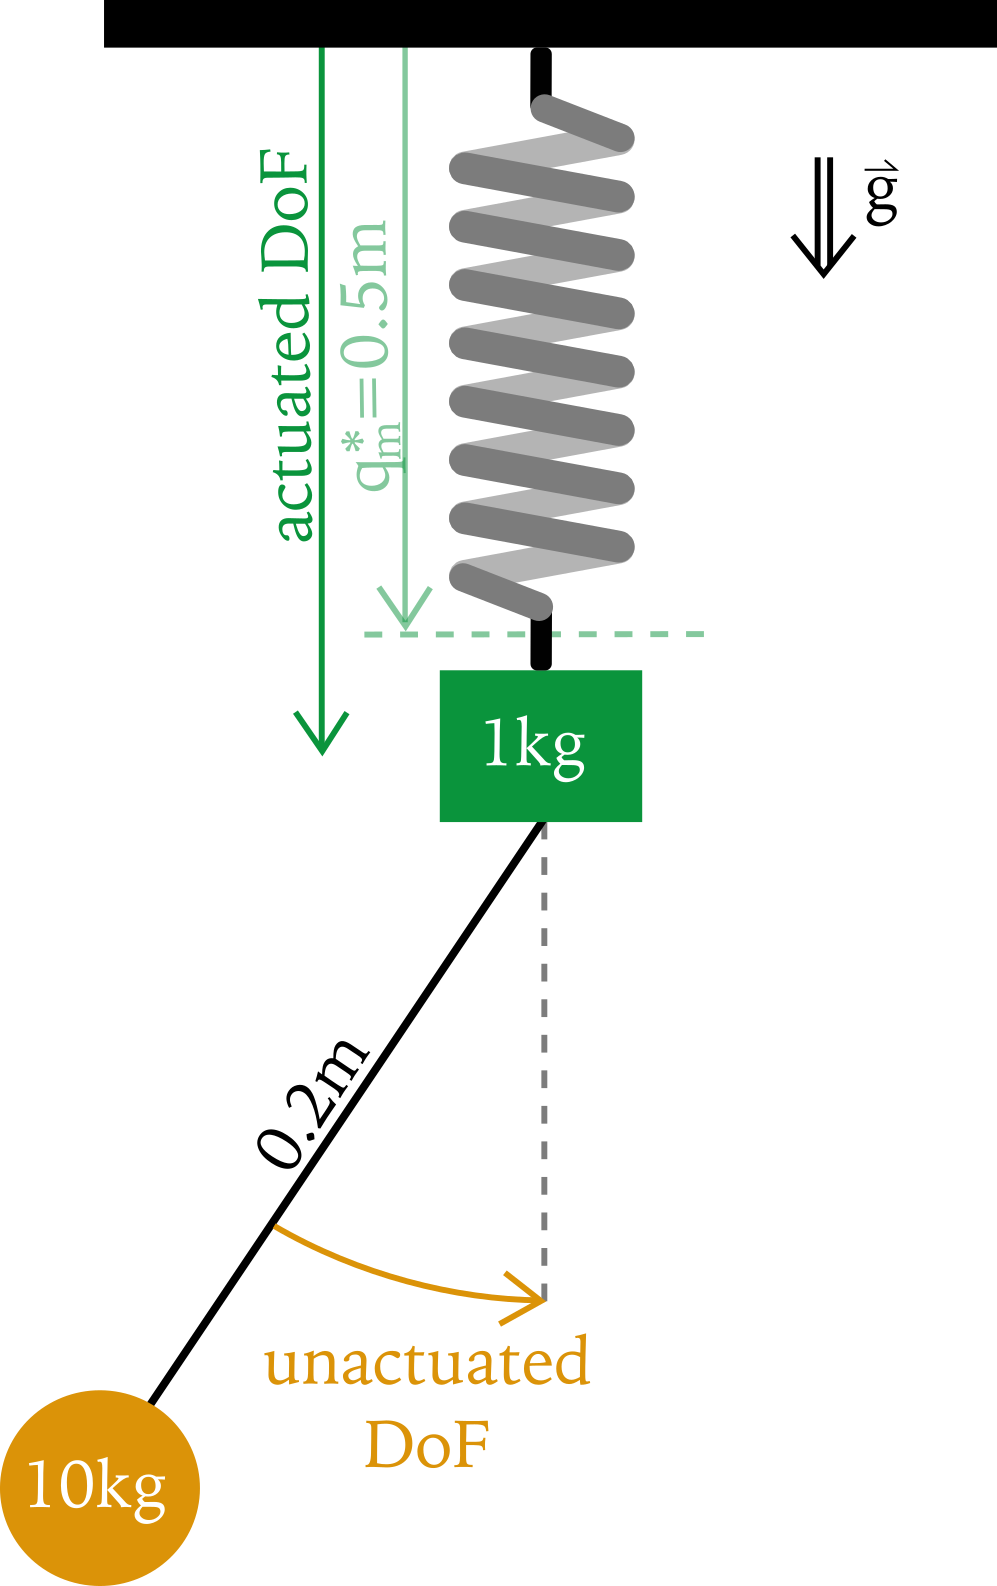
\includegraphics[width=0.35\columnwidth]{figures/Mass_Pendulum_Model.png}
\caption{Definition of the mass-pendulum-spring model.}
\label{fig:Mass_Pendulum_Model}
\end{figure*}

The spring is modelled by an external force of the following form:

\[
\begin{aligned}
F_{ext} = -k*Mass\_position
\end{aligned}
\addtag
\label{eq:f_ext}
\]
where k is the spring stiffness constant.


 
The first term of the objective function (Eq.~\ref{eq:ocp_Pendulum}) corresponds to the tracking of the mass position.
The second and third were added for control regularization.
The objective function, composed of Lagrange terms, was formulated as follow:


\[\label{eq:ocp_Pendulum}
\mathcal{J} = \underbrace{\int_{T/2}^T (q_{mass} + 0.5)^2~dt}_{TRACK\_STATE}  +~\omega_1 \underbrace{\int_{T/2}^T ~\tau^2~dt}_{MINIMIZE\_ TORQUE},
\]
\noindent with $q_{mass}$ the position of the mass, $\omega_1 = 1\times 10^{-6}$, T the duration of the movement and $\tau$ the force control of the mass.


The movement was first unactuated for $\SI{5}{s}$, then actuated for $\SI{5}{s}$ using a piece-wise constant force actuation.
Each phase was discretized using 51 shooting nodes.
At first, the mass is oscillating freely, then it stabilizes around the targeted position.
This example highlights the possibility to use OC to find activation patterns compensating external forces, here the spring force (Fig.~\ref{fig:Mass_Pendulum_Fext_graphs}).


\begin{figure*}[t!]
\centering
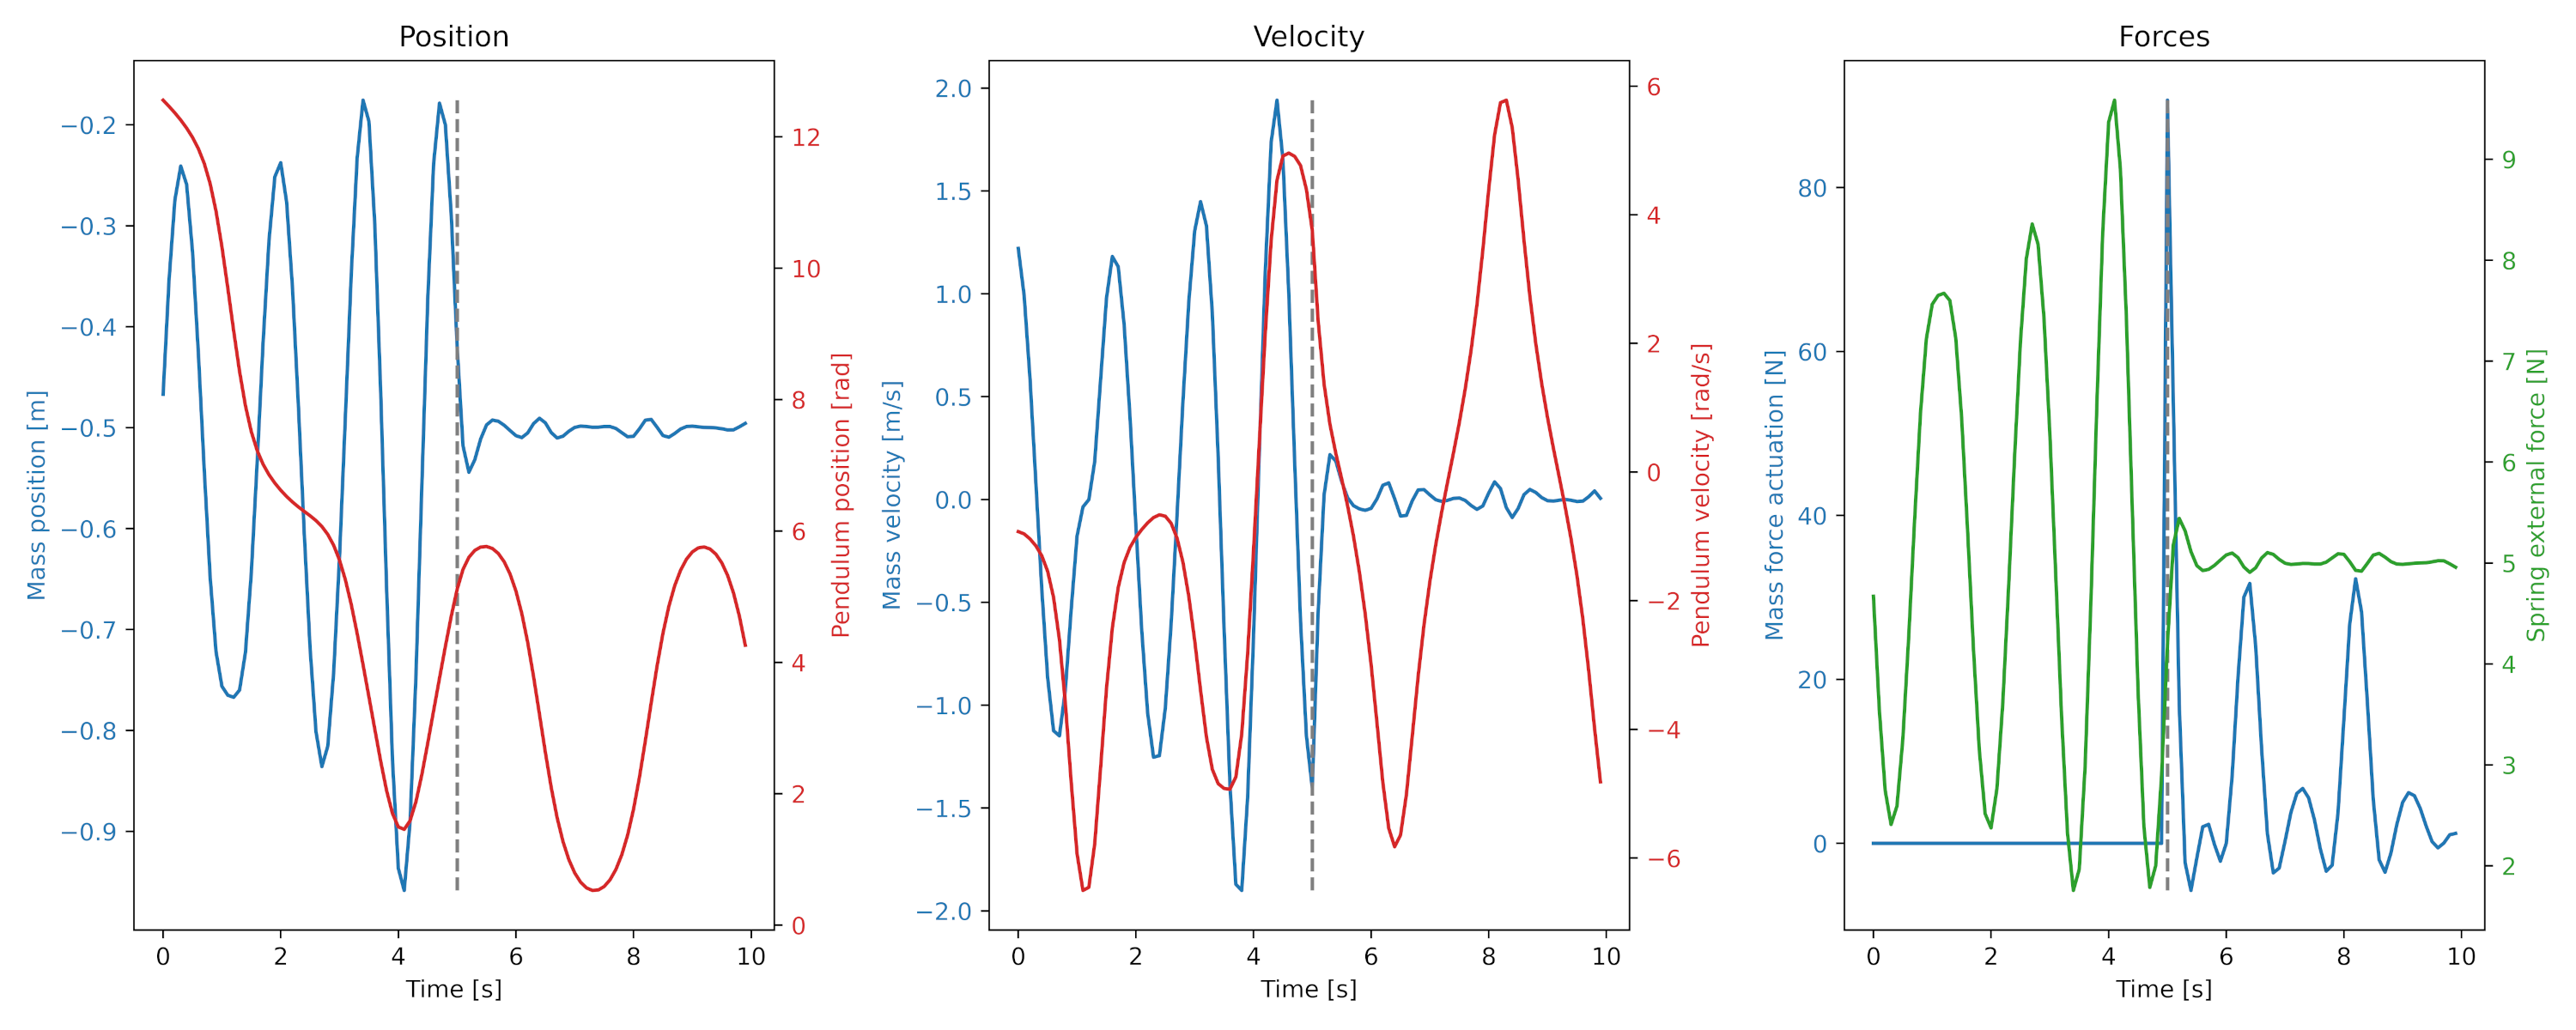
\includegraphics[width=\textwidth]{figures/Mass_Pendulum_Fext.png}
\caption{Optimal kinematics of the mass-pendulum-spring system. Gray dashed lines show the stage transition, blue lines are related to the mass, red lines are related to the pendulum and the green line is related to the spring.}
\label{fig:Mass_Pendulum_Fext_graphs}
\end{figure*}














